\chapter{Pupil Detection}
\label{chap:pupildetection}
\section{Ausgangslage}
\label{sec:current}
\section{Problemanalyse}

\section{Algorithm}
\subsection{Angle-Validation}
\label{sec:angleValidation}
To detect outliers it is necessary to find properties that differ strongly from the other transitions. One of those properties gets visible when the angle for each transition gets calculated with the neighbouring transitions. 

In figure \ref{fig:outlierOutside} a outlier lies on the bottom left corner of the image and outside of the pupil. The angle of the outlier is very small compared to angle of the neighbouring transitions. Those on the other hand have a greater angle than the other transition points. 

When a outlier is inside the pupil then the situation is reversed as visible in figure \ref{fig:outlierInside} where the outlier has a big angle and the adjacent transitions very small angles. 

\begin{figure}[H]
\begin{subfigure}{.5\textwidth}
	\centering
	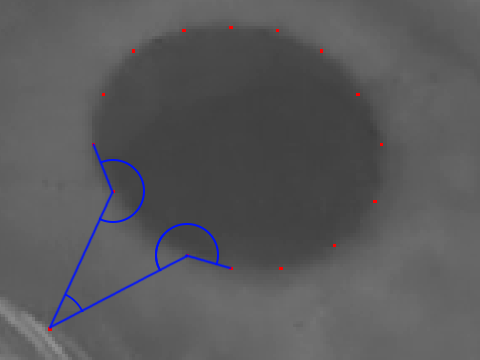
\includegraphics[width=.8\linewidth]{images/angle.png}
	\caption{Outlier outside Pupil}
	\label{fig:outlierOutside}
\end{subfigure}%
\begin{subfigure}{.5\textwidth}
	\centering
	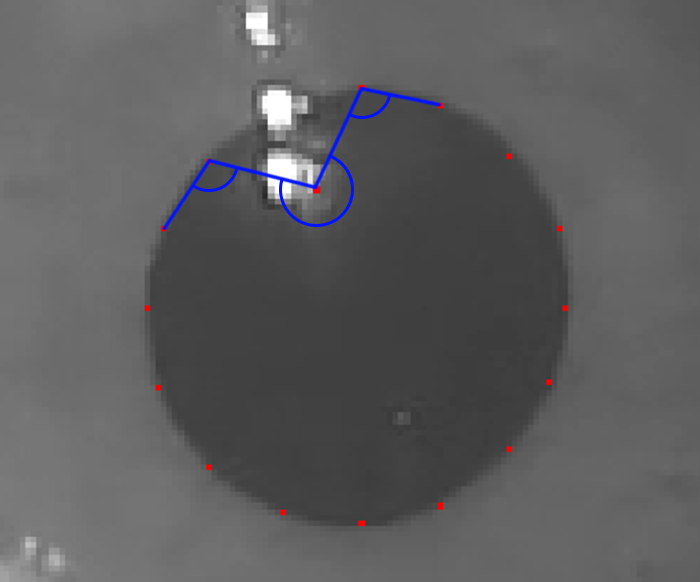
\includegraphics[width=.8\linewidth]{images/outlier_inner.png}
	\caption{Outlier inside Pupil}
	\label{fig:outlierInside}
\end{subfigure}
\caption{Angles between Transitions around Outliers}
\end{figure}

Multiple adjacent outliers differ in that it is not possible to make a clear statement what the angle will be. But the neighbours to the Outliers still have the same properties as described in the last paragraphs. For that reason an algorithm that wants to detect outliers should focus on detecting the neighbours of outliers.

\subsubsection{Overview of Algorithm}
\label{sec:descriptionOfAngleValidation}

The algorithm to detect outliers based on the angles between transitions involves four steps:

\begin{enumerate}
	\item Calculate angles
	\item Find 3 adjacent angles with small differences
	\item Categorize angles
	\begin{itemize}
		\item To big
		\item To small
		\item As expected 
	\end{itemize}
	\item Determine outliers
\end{enumerate}
\subsubsection{Calculate Angles}
\label{sec:calculateAngles}
The angle between the points is calculated with the vectors that stretch from the center point to the other points. For each vector the angle between the x axis and the vector is calculated with the atan2 function. The advantage of the atan2 over the conventional arctangent function is that it takes coordinates and returns the angle for the correct quadrant. The difference of the resulting two angles is the desired angle between the points. 

When the detected transitions are close to each other, measurement uncertainty can greatly affect the angles at such points. To mitigate that effect the angle for a point is only calculated with transitions that are distant enough.
\subsection{Find adjacent angles with small differences}
Context is important to categorize an angle. Only angles that are as expected do not always require context. This is the case when there are three adjacent angles that fall within a narrow range of each other and create context for the neighbouring angles.
\subsubsection{Categorize Angles}
The found context leads the way to iterate over every transition and categorize the angle within the context. This is done with the following rules:

\begin{figure}{}
	\centering
	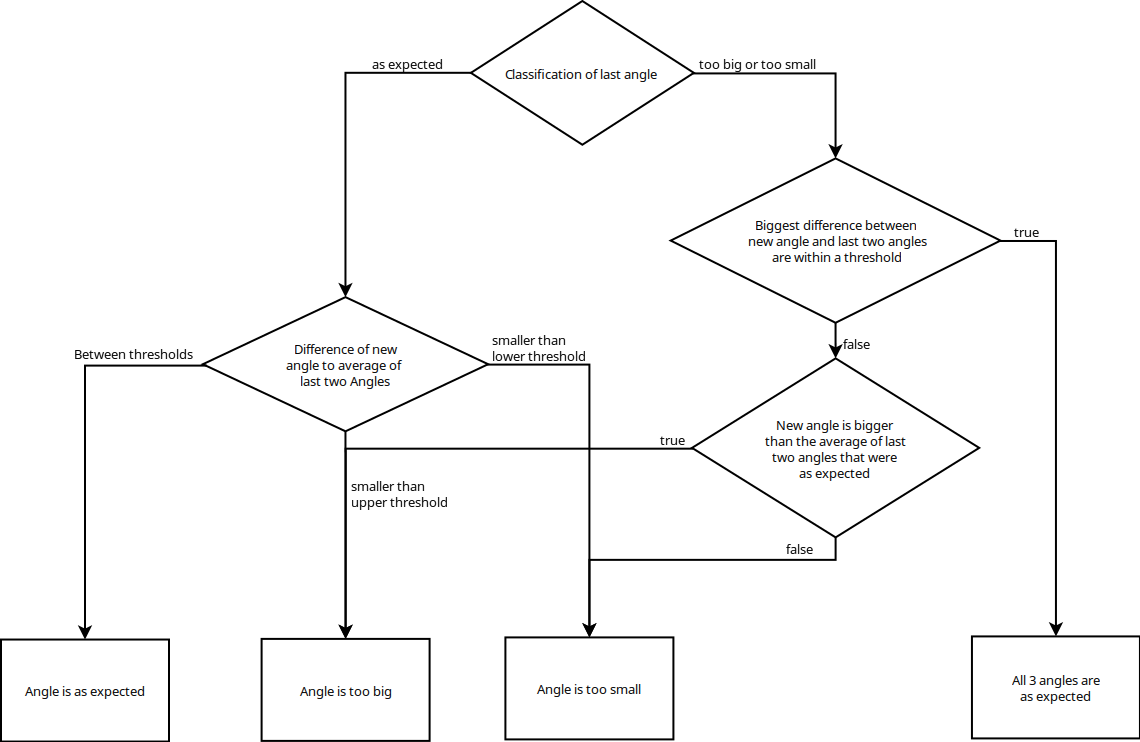
\includegraphics[width=1\linewidth]{images/angleclassification.png}
	\caption{Outlier inside Pupil}
	\label{fig:outlierInside}
\end{figure}
\subsection{Color of the Startpoint}
\label{sec:colorStartpoint}

\subsection{Randdetektion}
\label{sec:randdetektion}
\subsection{Gute Resultate ausn\"utzen}
\label{sec:guteResultate}

